%%%%%%%%%%%%%%%%%%%%%%%%%%%%%%%%%%%%%%%%%%%%%%%%%%%%%%%%%%%%%%%%%%%%%%%%%%%%%%%
%optimization.tex: Detector Optimization
%%%%%%%%%%%%%%%%%%%%%%%%%%%%%%%%%%%%%%%%%%%%%%%%%%%%%%%%%%%%%%%%%%%%%%%%%%%%%%%%
\chapter{Detector Design and Optimization}
\label{sec:optimization_chapter}
%%%%%%%%%%%%%%%%%%%%%%%%%%%%%%%%%%%%%%%%%%%%%%%%%%%%%%%%%%%%%%%%%%%%%%%%%%%%%%%%

\ac{EBEX} employed a kilopixel array of \ac{TES} bolometers, described in Section~\ref{sec:tes_bolometer}. 
%Several \ac{CMB} experiments have chosen to use \ac{TES} bolometers
These types of detectors were used on ground-based telescopes, like the Atacama Pathfinder Experiment and the South Pole Telescope \cite{Ruhl2004} \cite{Schwan2011}. 
We modified the design, described in Section~\ref{sec:detector_design}, in order to optimize the detectors to take advantage of the space-like environment in which \ac{EBEX} was flown.

%\textcolor{red}{Is it necessary/helpful to point to the sections here?}

%%%%%%%%%%%%%%%%%%%%%%%%%%%%%%%%%%%%%%%%%%%%%%%%%%%%%%%%%%%%%%%%%%%%%%%%%%%%%%%%
% TES Bolometer Theory {{{
%%%%%%%%%%%%%%%%%%%%%%%%%%%%%%%%%%%%%%%%%%%%%%%%%%%%%%%%%%%%%%%%%%%%%%%%%%%%%%%%
\section{Bolometer Theory}
\label{sec:tes_bolometer}
%%%%%%%%%%%%%%%%%%%%%%%%%%%%%%%%%%%%%%%%%%%%%%%%%%%%%%%%%%%%%%%%%%%%%%%%%%%%%%%%

%\textcolor{red}{Acronyms is failing us ... the figure descriptions are the first place they appear ... how do we fix this??? FIXED... BUT DON'T REMEMBER HOW :/}

%\textcolor{red}{Describe how a bolometer works. Power to temperature detector.}
% Need: cartoon. }


A bolometer, first invented by Langley in the late 1800s, is an absorber with some heat capacity weakly thermally coupled to a bath \cite{langley}.
%S. P. Langley. BOLOMETER. New York, The Society, 1880.
Figure~\ref{fig:bolometer_cartoon} is a schematic of a bolometer. 
Bolometers absorb power from radiation, via the heat capacitive element, and measure the resultant change in temperature with a thermistor. 
The bolometer's steady state power flow, $P$, from the absorber to the bath is described by
\begin{equation}
P = \overline{G} \left(T - T_{bath} \right) = \overline G \Delta T
\label{eq:gbar}
\end{equation}
where $\overline G$ is the average thermal conductance along the weak link and $\Delta T$ is the difference between the absorber and bath temperatures. 
The dynamic thermal conductance of the weak link is 
\begin{equation}
G \equiv \frac{dP}{dT}
\end{equation}
and is a function of position along the link. 
When additional power is deposited on the bolometer and absorbed, the temperature of the heat capacitive element increases and then the absorbed power dissipates to the bath via the link with a characteristic time constant of 
\begin{equation}
\tau = \frac{C}{G}
\end{equation}


\begin{figure}[htp]
\begin{center}
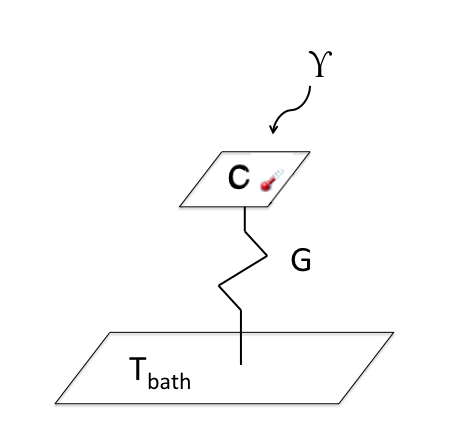
\includegraphics[height=2.5in]{figures/bolometer_cartoon}
\caption[Schematic of a bolometer]{Cartoon bolometer with incoming radiation, $\gamma$. There is an absorber, with heat capacity C, weakly coupled, with thermal conductance G, to a reservoir at $T_{bath}$. A thermistor measures the change in temperature due to the power absorbed. 
%\textcolor{red}{(Do you have time to add a thermometer or something to the chunk of heat capacity to show that's what you're measuring the temperature of?) Probably not. but did it anyhow.}
\label{fig:bolometer_cartoon} }
\end{center}
\end{figure}

\subsection{Transition Edge Sensors}

A \ac{TES} bolometer has a superconductor as its thermistor. 
A superconductor is a special material which has a normal resistance until it drops below its critical temperature, at which point its resistance drops to zero \cite{tinkham}.
%M. Tinkham, Introduction to Superconductivity, 2nd Ed., McGraw-Hill, NY, 1996, ISBN 0-486-43503-2
Figure~\ref{fig:r_vs_t} shows the resistance as a function of temperature for a superconductor. 
The \ac{TES} is called such because it is a sensor operated on the edge of its superconducting transition, where there is a steep change in resistance as a function of temperature. 

\begin{figure}[htp]
\begin{center}
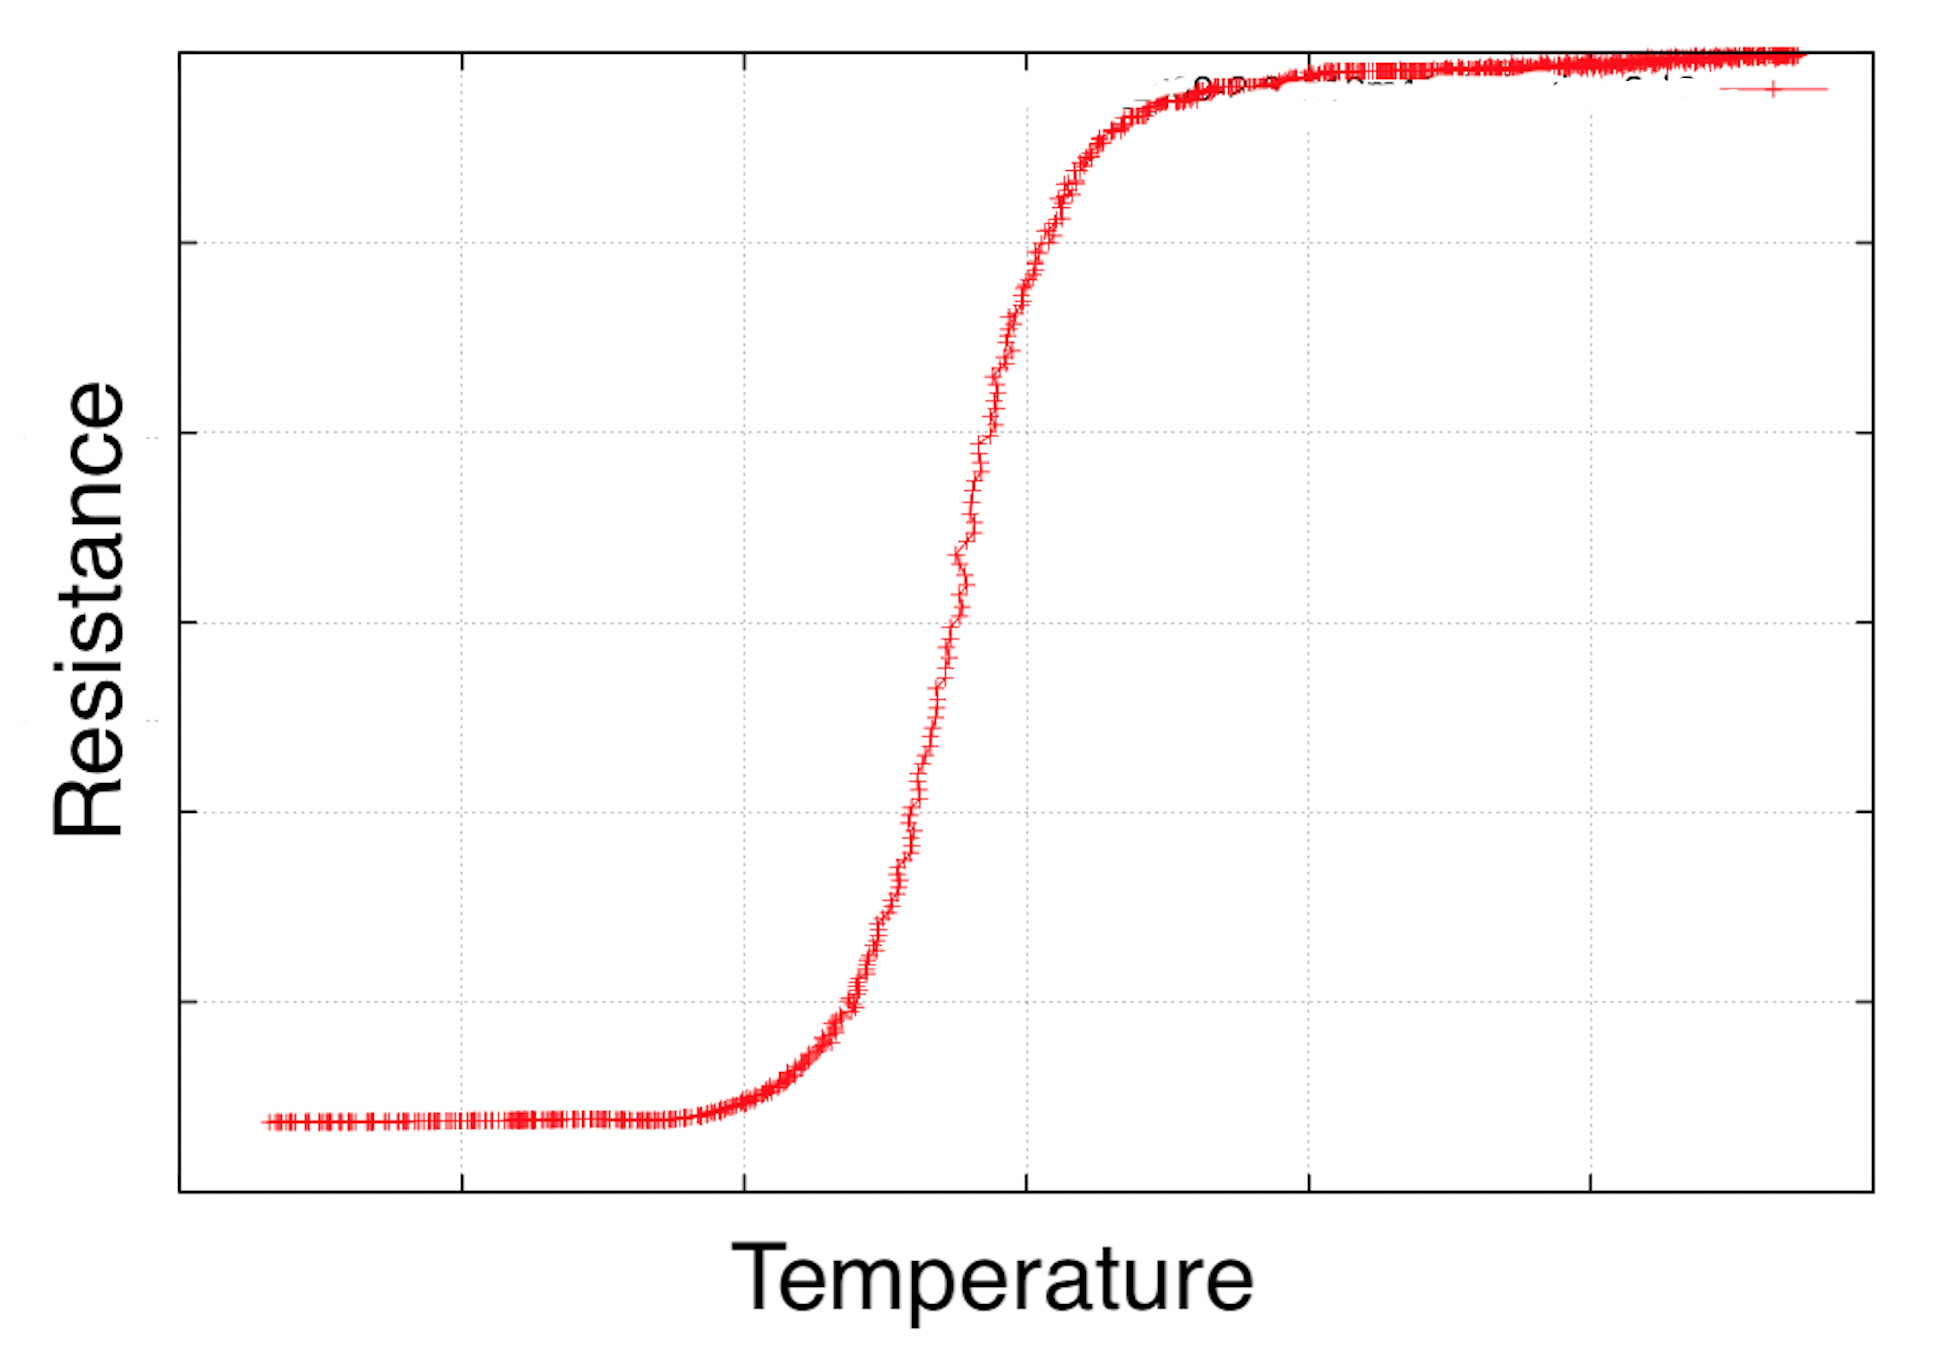
\includegraphics[height=2.5in]{figures/RvsT_for_thesis.png}
\caption[Typical resistance versus temperature curve for a superconductor]{Resistance versus temperature for an \ac{EBEX} \ac{TES} bolometer. As the temperature goes from high to low, the \ac{TES} goes from a finite normal resistance to superconducting with zero resistance. The region in between is the transition. The \ac{TES} is biased roughly in the middle (black dot) for operation. 
%\textcolor{red}{Make this figure prettier. Need to be able to read axes and their labels OR \textit{remove them}. Say where metal is normal and where it's superconducting and where it's transitioning and where the detector is operated.} 
\label{fig:r_vs_t} }
\end{center}
\end{figure}


\subsubsection{Negative Electrothermal Feedback}
%\textcolor{red}{Describe negative electrothermal feedback.}

%\textcolor{red}{For a moment here, just put down some words describing how it works. You can and will return to make it more technical and correct.}
To operate the detector, a voltage bias, $V_{bias}$, is applied across the \ac{TES}. 
The voltage bias provides Joule heating of $P_{elec} = V^{2}_{bias}/{R}$, where $R$ is the resistance of the \ac{TES}.
%In steady-state, there is a constant power flow from the detector to the bath. 
To understand the electrothermal feedback loop, i.e. what happens to the power dissipated in the bolometer when its temperature changes by a small amount, we take the derivative of the electrical power with respect to temperature, 
\begin{equation}
\begin{split}
\frac{dP_{elec}\left(T\right)}{dT} & = \frac{-V^{2}_{bias}}{R^2} \frac{dR}{dT} = - \frac{V_{bias}^2}{R} \frac{T}{R} \frac{dR}{dT} \frac{1}{T} \\
& = - \frac{P_{elec}\alpha}{T} %too many unnecessary steps ???
%\frac{dP_{total}}{dT} & = \frac{dP_{elec}\left(T\right)}{dT} + \cancel{\frac{dP_{rad}}{dT}} = \frac{-V^{2}_{bias}}{R^2} \frac{dR}{dT} \\
\end{split}
\end{equation}
where we define $\alpha$ to be a unitless measure of the slope of the resistance versus temperature curve,
\begin{equation}
\alpha \equiv \frac{d\log{R}}{d\log{T}} = \frac{T}{R} \frac{dR}{dT}
\end{equation}
Since the slope of the resistance versus temperature curve is positive for a \ac{TES}, the change in power is opposite in sign to the change of temperature. 
This negative electrothermal feedback holds the detector between normal and superconducting, at the edge of its transition. 

Qualitatively, the voltage bias is chosen such that the detector is heated just enough to hold the \ac{TES} between normal and superconducting. 
When the radiative load changes, the \ac{TES} warms (cools). 
This change in temperature moves the detector up (down) its R vs T curve. 
%That is, the resistance of the \ac{TES} increases (decreases) in response to an increase (decrease) in radiative load. 
In response to the increase (decrease) in resistance, the Joule heating decreases (increases) and the detector cools (warms). 
For small changes in temperature, this feedback holds the detector at the transition between normal and superconducting. 
The voltage bias is constant and so the excursions in resistance change the current through the detector and this is what we measure. 
%For flight, we calibrated on a known source in the sky to determine how much the current measured changed given a known amount of power from the sky.   %NOT RELEVANT

\subsubsection{Responsivity}

%To derive the detector responsivity we follow Richards~\cite{Richards} and Lee~\cite{Lee1998}.
To derive the detector responsivity we follow \cite{Richards} and \cite{Lee1998}.
The radiative signal absorbed by the detector consists of a steady state power~$P_{0}$ and a time varying signal of amplitude~$\delta P$ and frequency~$\omega$
\begin{equation}
P_{rad} = P_{0} + \delta P e^{i\omega t}
\end{equation}
The bolometer temperature is then also a function of time
\begin{equation}
T = T_{0} + \delta T e^{i\omega t}
\end{equation}
The total input power is the sum of the electrical power dissipated, $P_{elec}$ (including the first order change in electrical power due to the change in detector temperature), and the radiative power absorbed, $P_{rad}$,
\begin{equation}
%P_{in}\left(T\right) = P_{elec}\left(T\right) + P_{rad} = \frac{V^{2}_{bias}}{R\left(T\right)} - \frac{V_{bias}^2}{R\left(T\right)^2} \frac{dR}{dT} \delta T e^{i\omega t} + P_{0} + \delta P e^{i\omega t} 
P_{in} = P_{elec} + P_{rad} = \frac{V^{2}_{bias}}{R} - \frac{V_{bias}^2}{R^2} \frac{dR}{dT} \delta T e^{i\omega t} + P_{0} + \delta P e^{i\omega t} 
\label{eq:pin}
\end{equation}
The total output power is the steady state power flow to the bath, Equation~\ref{eq:gbar}, plus the time varying power to the bath plus the time varying power stored in the heat capacity
\begin{equation}
P_{out} = \overline{G}\Delta T + G \delta T e^{i\omega t} + i\omega C \delta T e^{i\omega t}
\label{eq:pout}
\end{equation}
%shaul didn't like the following, but I think it was fine...
%Conservation of power equates Equation~\ref{eq:pin} and Equation~\ref{eq:pout}. 
Power is conserved, so Equation~\ref{eq:pin} equals Equation~\ref{eq:pout}.
The time-independent portion is 
\begin{equation}
P_{0} + \frac{V^{2}_{bias}}{R} = \overline{G}\Delta T 
\label{eq:p_time_independent}
\end{equation}
%This equation describes the steady state power flow and determines the detector's operating temperature. 
The time-dependent portion is
\begin{equation}
\delta P - \frac{V_{bias}^2}{R^2} \frac{dR}{dT} \delta T = G \delta T + i\omega C \delta T \label{eq:p_time_dependent}
\end{equation}
It describes the change in power due to a small change in temperature
\begin{equation}
\begin{split}
\frac{\delta P}{\delta T} & = \frac{V_{bias}^2}{R^2} \frac{dR}{dT} + G + i\omega C \\
%& = \frac{V_{bias}^2}{R} \frac{T}{R} \frac{dR}{dT} \frac{1}{T} + G + i\omega C \\
& = \frac{P_{elec}\alpha}{T} + G + i\omega C \\
\end{split}
\label{eq:dp_dt}
\end{equation}
%where we define $\alpha$ to be a unitless measure of the slope of the resistance versus temperature curve,
%\begin{equation}
%\alpha \equiv \frac{d\log{R}}{d\log{T}} = \frac{T}{R} \frac{dR}{dT}
%\end{equation}
%\textcolor{red}{Help! I've confused myself. this equation looks like we have positive feedback???}
%Since the slope of the resistance versus temperature curve is positive for a \ac{TES}, the change in power is opposite in sign to the change of temperature. 
%This negative electrothermal feedback holds the detector at the edge of its transition. 
The electrothermal feedback loopgain is the change in electrical power in response to the small absorbed radiative signal relative to the signal amplitude
\begin{equation}
\mathscr{L} \left( \omega \right) = - \frac{\delta P_{elec}}{\delta P} = \frac{P_{elec} \alpha}{GT(1+i\omega \tau_{0})} = \frac{\mathscr{L}}{1 + i \omega \tau_{0}}
\end{equation}
The DC value of the loopgain is 
\begin{equation}
\mathscr{L} = \frac{P_{elec}\alpha}{GT}
\label{eq:dc_loopgain}
\end{equation}
and it rolls off with a time constant of $\tau_{0} = C/G$.
The current responsivity of the detector is the change in current we measure for a given amount of radiative power absorbed
\begin{equation}
S_{I} \equiv \frac{\delta I}{\delta P} %= - \frac{1}{V_{bias}} \frac{\delta P_{elec}}{\delta P} 
= - \frac{1}{V_{bias}} \left( \frac{\mathscr{L}}{\mathscr{L}+1} \right) \left( \frac{1}{1+i\omega \tau_{eff}} \right)
\label{eq:responsivity}
\end{equation}
where $\tau_{eff} = \tau_{0}/ ( 1 + \mathscr{L})$ is the effective time constant, sped up by electrothermal feedback. 
Note, for the \ac{DfMUX} system, there is an additional factor of $\sqrt{2}$ in the current responsivity due to demodulation.
%IF YOU HAVE TIME, COME BACK HERE AND EXPLAIN MORE




%The total power in is the radiative power plus the electrical bias power plus the electrical power change due to the bolometer temperature change.
%The total power out is the steady state power to the bath plus the time varying power to the bath plus the power stored in the heat capacity. 
%The total power flow is \cite{Lee1998}
%\begin{equation}
%P + \delta P e^{i\omega t} + \frac{V_{bias}^2}{R} - \frac{V_{bias}^2}{R^2} \frac{dR}{dT} \delta T e^{i\omega t} = \overline{G}\Delta T + G \delta T e^{i\omega t} + i\omega C \delta T e^{i\omega t}
%\end{equation}



%mathematical description of a small incident signal. i.e. poptical = psteady + ptimevarying
%\textcolor{red}{What are the other essential pieces to explaining how a bolometer works?
%Responsivity. i.e. 
%Dynamic Range?
%you've touched on power flow and negative electrothermal feedback. 
%we haven't touched on how power depends on bath temperature and n.
%dynamic range? 
%bandwidth? 
%"We quantify the dynamic range, responsivity, sensitivity, and bandwidth of a TES
%bolometer by following [25]." lanting
%[25] S. Lee, J. M. Gildemeister, W. Holmes, A. T. Lee, and P. L. Richards. Voltage-Biased
%Superconducting Transition-Edge Bolometer with Strong Electrothermal Feedback Operated
%at 370 mK. Applied Optics, 37:3391�3397, June 1998.
%}



%\textcolor{red}{derive it? that's what I want you to do ... at the very least, spell out how it's done. barfing equations on paper isn't my style.}

%\textcolor{red}{Does it make sense to talk about the four sources first and then provide the expression for total NEP? Or to first provide the expression and then derive/talk about each source? It doesn't matter! Just do one!}

%\textcolor{red}{Figure out how to properly add : 
%Kyle's thesis details need to be added
%Mather 1982 applied optics bolometer noise paper to bibfile and reference. 
%Also add Lamarre, "Photon noise in photometric instruments at far-infrared and submillimeter wavelengths", applied optics, vol 25, no 6, 15 march 1986 (he's not there)
%langley - S. P. Langley. BOLOMETER. New York, The Society, 1880.
%tinkham - M. Tinkham, Introduction to Superconductivity, 2nd Ed., McGraw-Hill, NY, 1996, ISBN 0-486-43503-2
%}

\subsection{Noise Equivalent Power}

The sensitivity of the detectors is quantified by their \ac{NEP}. 
%should I instead say sensitivity of the instrument?
\ac{NEP} is defined as the absorbed power required to produce a signal-to-noise ratio of one in a  bandwidth of one~Hz. 
For purposes of brevity, we will also refer to the \ac{NEP} simply as noise. 
% \ac{NEP} is a measure of signal-to-noise, we will use the terms noise and \ac{NEP} interchangeably. 
%\textcolor{red}{That sounds like a stupid idea.}
There are four contributors to the \ac{TES} bolometer \ac{NEP}: electronic readout noise, Johnson noise, phonon noise, and photon noise. 
%not important?
%Note, sometimes \ac{NEP} is instead defined as the \textit{incident} power required to produce a signal-to-noise ratio of one in an electrical bandwidth of one~Hz, \textcolor{red}{cite who??}.
The total predicted detector \ac{NEP}, $N$, is given by 
\begin{equation}
%N^{2} = N_{photon}^2 + N_{phonon}^2 + \frac{1}{S_I^2} \left( N_{Johnson}^2 + N_{readout}^2 \right)
N^{2} = N_{photon}^2 + N_{phonon}^2 + N_{Johnson}^2 + N_{readout}^2
\end{equation}
\begin{equation}
= 2h\nu P_{rad} + \xi \frac{P_{rad}^2}{\Delta \nu} + \gamma 4k_{B} T^2 G + \frac{1}{S_I^2} \left(\frac{4k_{B}T}{R} + N_{readout}^2 \right)
\label{eq:nep}
\end{equation}
where $h$ is Planck's constant, $\nu$ is the center of the observation frequency band, $P_{rad}$ is the radiative power absorbed by the bolometer, $\xi$ is a unitless number between zero and one quantifying the contribution of photon correlation noise, $\Delta \nu$ is the width of the observation frequency band, $\gamma$ is a unitless number between zero and one accounting for the temperature gradient along the link from the \ac{TES} to the bath, $k_{B}$ is Boltzmann's constant, $T$ is the \ac{TES} temperature, $G$ is the bolometer dynamic thermal conductance, $S_{I}$ is the bolometer current responsivity, and $R$ is the \ac{TES} resistance \cite{Mather1982}. 
\ac{TES} bolometers have been developed such that the the fundamental limit of the \ac{NEP} can be set by the photon arrival statistics, i.e. background limited. 
We wanted to create an instrument with background noise limited \ac{TES} bolometers. 

%YOU TALK ABOUT THIS LATER. 
%Both the Johnson and readout noise will have been referred to current through the \ac{SQUID}, so they are divided by the current responsivity, 
%%\begin{equation}
%%S_I = \frac{dI}{dP} = \frac{-\sqrt{2}}{V_{bias}}
%%%not \equiv ?
%%\end{equation}
%in order to convert them to units of $W/\sqrt{Hz}$. 

\subsubsection{Readout Noise}

The electronic readout noise is due to current and voltage fluctuations in the readout electronics, i.e. the carrier, nuller, and demodulator circuits, schematic shown in Figure~\ref{fig:dfmux}. 
The electronic components were sourced with the requirement that their noise, added in quadrature, provided a subdominant contribution to the \ac{NEP}. 
The largest contributors were the 4.2~K \ac{SQUID}s and their room temperature first stage operational amplifiers. 
Measurements of the electronic and readout noise are discussed in Section~\ref{sec:dark_noise} and Section~\ref{sec:flight_noise_performance}.
%COME BACK TO THIS IF YOU HAVE TO TIME
%\textcolor{red}{should we point to our noise discussions later? I guess do this. And in that later section, be sure to reference franky's thesis? and/or dfmux papers??}
%\textcolor{red}{Were you thinking you want to say something about how there's no nice succinct expression for readout \ac{NEP}, but rather a lengthy expression adding all the numbers from the manufacturers in quadrature?}
%There is not a nice, succinct expression for the readout electronics \ac{NEP}, but rather a lengthy expression adding all the numbers from the manufacturers in quadrature and referencing each noise source to current through the \ac{SQUID}. 
%The measurement and the theory agree to within $13\%$ of each other. 

\subsubsection{Johnson Noise}

The Johnson noise is due to the thermal agitation of the electrons in the \ac{TES}. 
As a voltage-referred noise, in units of $V^2/Hz$, the Johnson noise \ac{PSD} is $4k_{B}TR$,
%\begin{equation}
%v^2 = 4k_{B}TR
%\label{eq:johnson_v}
%\end{equation}
where $k_{B}$ is Boltzmann's constant, $T$ the temperature of the resistor, and $R$ the resistance \cite{PhysRev.32.97}.
Note, this voltage noise source is present regardless of any applied voltage.
%\textcolor{red}{Should this be an equation? Should we derive it? Whatever you do, reference!}
In order to convert the Johnson noise from our \ac{TES} to a current-referred noise, we divide the voltage noise \ac{ASD} by R, $\sqrt{4k_{B}TR}/R = \sqrt{4k_BT/R}$. 
For \ac{NEP}, in order to convert from $A/\sqrt{Hz}$ to $W/\sqrt{Hz}$, we divide the current noise by the bolometer's current responsivity, $S_{I} = dI/dP$. 
The Johnson \ac{NEP} is thus
\begin{equation}
N_{Johnson} =  \frac{1}{S_I} \sqrt{ \frac{4k_{B}T}{R}}
\label{eq:johnson}
\end{equation}
%don't love this explanation, but we're just looking for good enough.

\subsubsection{Phonon Noise}

The phonon noise is due to the motion of the thermal carriers, phonons, along the weak thermal link. 
This random thermodynamic energy flow gives rise to the phonon \ac{NEP},
\begin{equation}
N_{phonon} = \sqrt{\gamma 4k_{B} T^2 G}
\label{eq:phonon_nep}
\end{equation}
where $k_{B}$ is Boltzmann's constant, $T$ is the temperature of the \ac{TES}, and $G \equiv dP/dT$ is the dynamic thermal conductance along the weak link \cite{Mather1982}. 
%mather says it "is readily shown from thermodynamics that this power flow ...". BUT. it's not obvious to me. Sadly. there's not time to understand this right now. You can return if you have the luxury to do so. 
 $\gamma$ is a unitless number between zero and one which describes the temperature gradient along the thermal link from the \ac{TES} to the bath  
\begin{equation}
\gamma \equiv \frac{\int_{T_{bath}}^{T} \left( \frac{t\kappa(t)}{T\kappa(T)}\right)^2 dt}{\int_{T_{bath}}^{T} \frac{\kappa(t)}{\kappa(T)} dt} 
\label{eq:gamma_integral}
\end{equation}
where $\kappa$ is the thermal conductivity, $T$ is the bolometer temperature, and $T_{bath}$ is the bath temperature \cite{Mather1982}. 
When we assume $\kappa(T) = \kappa_0 T^n$ and also assume the bolometer temperature $T$ is equal to its critical temperature $T_c$, then
\begin{equation}
\gamma = \frac{n+1}{2n+3} \frac{1-\left(\frac{T_{bath}}{T_c}\right)^{2n+3}}{1-\left(\frac{T_{bath}}{T_c}\right)^{n+1}}
\label{eq:gamma}
\end{equation}

%\textcolor{red}{shouldn't we have said somewhere the dynamic thermal conductance is $G \equiv dP/dT$ ? Do you want to relate $\kappa$ to $G$?}

\subsubsection{Photon Noise}

%The photon noise is due to the particle nature of photons and the Poisson statistics which govern their arrival. %This is only true if you're only talking about the first term of the photon noise.
The photon noise is due to the particle nature of photons and the statistics which govern their arrival. 
%YOU CAN COME BACK AND EXPLAIN THIS MORE IF YOU HAVE TIME
Quantifying the fluctuations in the absorbed energy (via boson statistics) and integrating over the radiation bandwidth, the photon \ac{NEP} is
\begin{equation}
N_{photon}^2 = 2 \int h \nu P_{\nu} d\nu + \xi \int \frac{P_{\nu}^{2}c^2}{A\Omega\nu^2} d\nu
\label{eq:photon_nep}
\end{equation}
where $h$ is Planck's constant, $\nu$ is the frequency of the radiation, $P_{\nu}$ is the absorbed spectral power, and $\xi$ is the so-called correlation factor \cite{Richards}. 
%this $P_{\nu}$ was a sticking point for you when you were trying to understand this. are you SURE you're using the correct words??? Eh. both richards and lammare call it spectral power. good enough for now. 
If we assume the spectral power is roughly constant over a small bandwidth and that we have a diffraction limited beam so the throughput is $A\Omega = \lambda^2$, where $\Omega$ is the solid angle of a wave after passing through a circular aperture of area $A$ and $\lambda$ is the wavelength of the incident light, then the photon \ac{NEP} becomes
\begin{equation}
N_{photon} = \sqrt{2h \nu P_{rad} + \xi \frac{P_{rad}^{2}}{\Delta\nu}}
\end{equation}
%YOU DERIVED THIS WITH SHAUL, BUT YOU FORGOT. I WISH YOU HAD THE TIME TO DO IT AGAIN. 
%Also, other people say what $P_{\nu}$ is for a blackbody, but if I recall, I was confused because the exact shape is not relevant! (simply that it doesn't change much for small bandwidth)
where $P_{rad}$ is the radiative power absorbed and $\Delta\nu$ the observation frequency bandwidth. 


%The \ac{EBEX} optics were designed to provide a diffraction limited beam. 
%I'D LIKE TO REFERENCE SOMETHING/ONE HERE
 
The first term of the photon \ac{NEP} is often referred to as shot noise. 
The second term is only relevant if the photon arrivals are correlated, that is if the photons tend to arrive in bunches. 
This is called photon correlation or bunching noise. 
The degree to which this second photon noise term contributes to the bolometer \ac{NEP} is not agreed upon \cite{Richards}. 
%\textcolor{red}{who says this? richards. and he says van vliet and mather do one thing and pike and lamarre do other things. can I just reference richards? or do I have to refer to all these other folks?}
This disagreement is encapsulated in the factor of $\xi$ which is multiplied by the noise one would have in the case of complete correlation.
$\xi$ can take on a value between zero (no correlation) and one (completely correlated).
Lamarre writes, the photon correlation factor when the "beam is produced by an incoherent source and is uniformly distributed over the beam throughput, which is large with respect to the etendue of coherence $\nu^{2}/c^{2}$" is completely different than the photon correlation factor in the case of telescopes "observing sources with angular diameters much smaller than the diffraction pattern" \cite{Lamarre}. 
While our source, the \ac{CMB}, is incoherent and uniformly distributed over the beam throughput, the beam throughput is equal to (so not large with respect to) the etendue of coherence. 
It is not clear what the true value of $\xi$ should be for \ac{EBEX}.

%\textcolor{red}{do you have anything else to say about shot noise?
%does it make sense to do $N_{source}$ or $N_{source}^2$?
%I'm not sure you've correctly explained how we get from voltage noise to current noise for johnson.
%}

%\textcolor{red}{(IF THERE IS TIME, reference more papers on the xi disagreement.)}



%%%%%%%%%%%%%%%%%%%%%%%%%%%%%%%%%%%%%%%%%%%%%%%%%%%%%%%%%%%%%%%%%%%%%%%%%%%%%}}}



%%%%%%%%%%%%%%%%%%%%%%%%%%%%%%%%%%%%%%%%%%%%%%%%%%%%%%%%%%%%%%%%%%%%%%%%%%%%%%%%
% Detector Design Modifications for Space-Like Environment {{{
%%%%%%%%%%%%%%%%%%%%%%%%%%%%%%%%%%%%%%%%%%%%%%%%%%%%%%%%%%%%%%%%%%%%%%%%%%%%%%%%
\section{Detector Design}
\label{sec:detector_design}
%%%%%%%%%%%%%%%%%%%%%%%%%%%%%%%%%%%%%%%%%%%%%%%%%%%%%%%%%%%%%%%%%%%%%%%%%%%%%%%%

%\textcolor{red}{Sure would be nice if you had more time to talk about how the detectors are fabricated. Go ahead and just reference Ben's thesis for now?}

The \ac{EBEX} bolometers were fabricated on a silicon device wafer, the thickness of which, $\lambda/4$, was determined by the center of the observation band. 
The device wafer was glued to a thick silicon backing wafer for mechanical stability \cite{Westbrook2014}.
The left panel of Figure~\ref{fig:bolo_and_bling} is a photograph of a single \ac{EBEX} bolometer. 
The absorber, to which radiation coupled, was a 1~$\mu m$ thick silicon nitride spider web. 
The silicon nitride was deposited on the device wafer and a silicon etch carved away the silicon underneath so the web was actually suspended in space.
The link to the bath was provided by eight legs which attached the web to the silicon wafer. 
The heat capacity was provided by a gold waffle, called bling, in the center. 
The \ac{TES} itself was an AlTi bilayer in the shape of a 19 x 19~$\mu m^{2}$ square located towards the center of the bling. 
The left edge of the bilayer overlapped the bling, right panel of Figure~\ref{fig:bolo_and_bling}, providing the thermal coupling between the absorber and the \ac{TES}.

\begin{figure}[ht!]
\begin{center}
%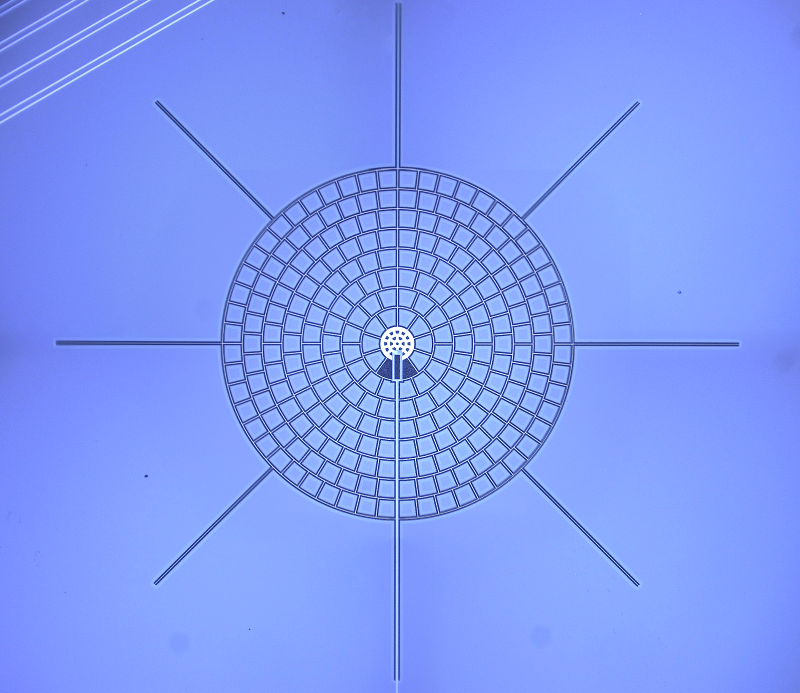
\includegraphics[width=0.49\columnwidth]{figures/bolometer_photo.png}
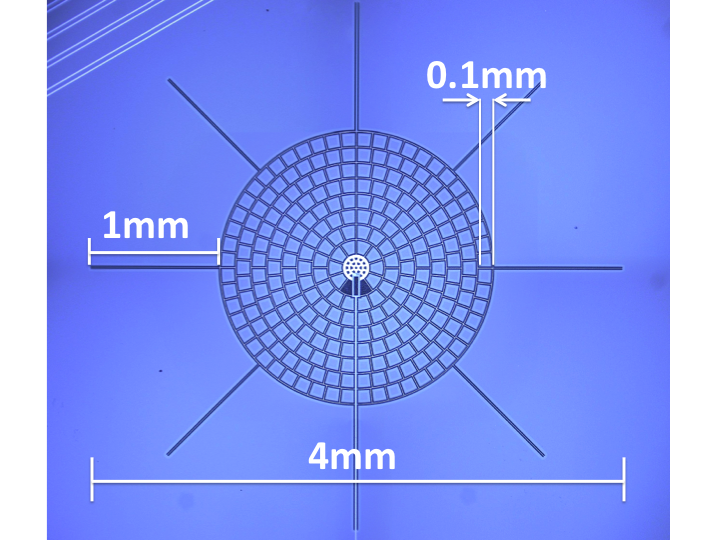
\includegraphics[width=0.49\columnwidth]{figures/fullpixel1_v4_small_annotated.png}
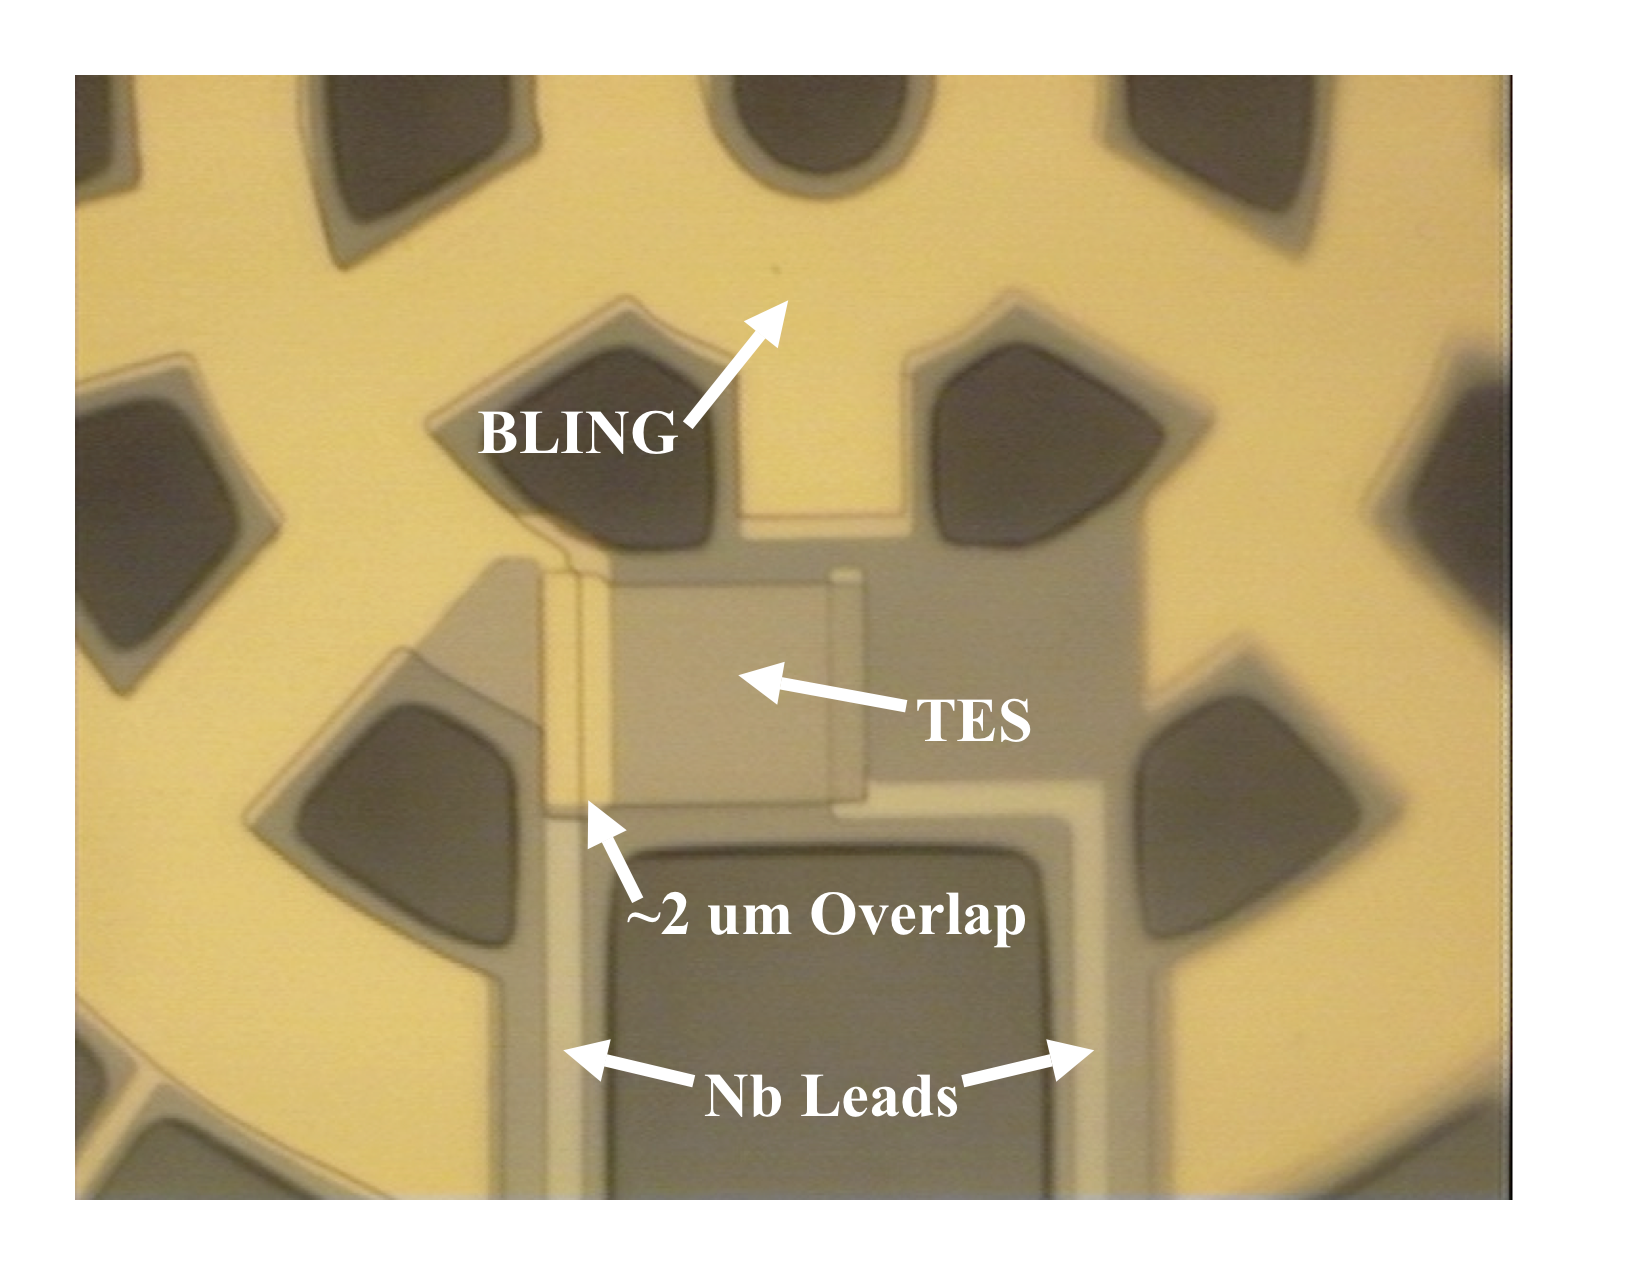
\includegraphics[width=0.45\columnwidth]{figures/EBEX_BLINGTES_Annotated.png}
\caption[EBEX TES bolometer photographs]{Left: One \ac{EBEX} 150~GHz spiderweb \ac{TES} bolometer. The light blue is the silicon wafer on which the detectors were fabricated. The dark blue is open space where the silicon was etched away. Running above the center of the etched out area are the thin silicon nitride strings of the spider web. The spider web is attached to the wafer at the end of each of the spokes. The gold waffle bling in the center provides the heat capacity. Right: A zoom of the bling and the \ac{TES}. The \ac{TES} is a square near the middle of the bling and is coupled to the bling via the overlap on its left side. The signal travels out the niobium leads to bond pads at the wafer's edge. Both figures courtesy of Benjamin Westbrook. 
\label{fig:bolo_and_bling} }
\end{center}
\end{figure}

%\textcolor{red}{How do I properly say this is Ben's not mine?? Looks like others don't really mention where the figures they didn't make are from ... Hmmm.}

%\textcolor{red}{LET GO. Why do you want to say this anyhow? In the first generation wafers, the bling was a simple circle, but in later designs, the bling was a waffle because it coupled better the absorbed power to the \ac{TES}.}


%Discuss target detector parameters. Be very clear about which changes were made to fabrication process in order to optimize the detector sensitivity for a space-like environment and for EBEX.

\subsubsection{Normal Resistance} 

The \ac{TES} bolometer response would be unstable if it were underdamped or had exponentially increasing oscillations \cite{Enss2005}. 
The goal was to ensure the detector, when biased in the transition, remained in the stable regime.  
The stability of the detector depended on the value of the normal resistance. 
In order to be stable, the bolometer's LCR filter bandwidth, $\Delta B = R_{bolo}/(2\pi L)$, needed to exceed the \ac{TES}' effective thermal bandwidth by a factor of 5.8 \cite{Irwin1998b}. 
With our inductors of 24~$\mu H$ and expected thermal time constants on the order of 10~ms, the target normal resistance for all bands was 1.5~$\Omega$, Table~\ref{tab:Design_Params}.
%I DID SOME CALCULATIONS, BUT MY NUMBERS DON'T QUITE WORK OUT IN A WAY THAT I UNDERSTAND. COME BACK HERE IF YOU HAVE TIME. 
 
%where the detector electrical bandwidth, determined in part by the resistance, exceeded the \ac{TES} effective thermal bandwidth by at least a factor of 5.8 (CITE PAPER). 

The electrical cross-talk was also a function of the bolometer resistance. 
In designing the electronics, we required the electrical cross-talk be subdominant to the optical cross-talk, due to beam side-lobes and radiation leakage within the detector integration cavity, which is typically at a level of $\sim$1\% \cite{Dobbs2011} . 
%There is electrical cross-talk between detectors due to the modulation of the detector resistance which results in the modulation of the carrier bias. 
%The level of this leakage is approximated by calculating the current modulation due to the neighboring bolometer's carrier bias leaking relative to the on-resonance current modulation for a bolometer ~\cite{Dobbs2011}
This electrical cross-talk was estimated by Dobbs, et al. ~\cite{Dobbs2011} to be
\begin{equation}
\left| \frac{R_{bolo}^2}{(2\Delta \omega L)^2} \right|
\end{equation}
%see page 100 of notebook for calculation
For \ac{EBEX} we had inductors of $L_{EBEX} = 24~\mu H$ and frequency spacing of at least $\Delta \omega = 2\pi \cdot 60~kHz$. %$\Delta \nu = 60~kHz$. %
%The lower bias frequencies have 60~$kHz$ spacing, but the higher bias frequencies (the lower capacitance values) are spaced by 80~$kHz$. 
%This is because the change more (in absolute value)and the resonant frequency spacing is larger than predicted.)
For a detector dropped to 85\% in the transition, a normal resistance of 1.5~$\Omega$ resulted in predicted electrical cross-talk at a level of 0.5\%.






%having a normal resistance of 1.9~$\Omega$ instead of 1.5~$\Omega$ results in a bias leakage increase of 60\%, increasing the cross-talk from 0.5\% to 0.8\%

%The consequences of overshooting this value, as is the case for many of the 150~GHz detectors, are an increase in the detector voltage bias leakage, which is proportional to $R^2$ \cite{dobbs_revSciInst_2012}, and a decrease in the loopgain, which is inversely proportional to R. 
%% if R is higher, then johnson current noise is decreased since it goes like 1/sqrt(R)
%% if R is higher, then stability requirement has R/(2*pi*L) > 5.8/tau_tes is more satisfied
%For a detector dropped to 85\% in the transition, having a normal resistance of 1.9~$\Omega$ instead of 1.5~$\Omega$ results in a bias leakage increase of 60\%, increasing the cross-talk from 0.5\% to 0.8\%, and a loopgain decrease of 30\%. 
%The consequence of undershooting the normal resistance, as is the case for many of the detectors on wafer 410-28, is an increase in the Johnson current noise. The Johnson noise is proportional to $1/\sqrt{R}$, so that noise term increases by 20\% given a value of 1.0~$\Omega$ instead of 1.5~$\Omega$.
%\comred{Assume detector optimization explains what about the electronics set our target to be 1.5~$\Omega$? Ben says "The requirement is really ~1.25 because what actually matters is Rtes in transition for the L/R requirement.  So depending on how deep we get in to the transition we could start anywhere just above 1.2 Ohms to operate at 0.88 to 1.0 Ohms." BUT. When determining which Rfrac to tune to, we didn't do this calculation. Rather, we noted, in general, below 80\% $R_{start}$, we had (not well understood) excess noise and so opted to go to 85\%. What I'm trying to say is, in practice, the operating fracRn value was not chosen carefully on a bolo by bolo basis or even a wafer by wafer basis to achieve a specific L/R. Explain the consequence of having a higher or lower normal resistance, e.g. 150s and one of the 410s (was it the 410 that operated or the 410 that was saturated?)? Ben says "Increased johnson noise and possibly bolo stability.  However, I'm not sure if either of these effects were detected in the wafers in test cryostats, Palestine, or flight."}




\subsubsection{Transition Temperature} 

%\textcolor{red}{Need to generate: plot of phonon noise as a function of critical temperature, given a fixed ebex bath temperature of 260~mK.}

%\textcolor{red}{For a thermal conductance that follows a power law, what kind of material is n=1 and what about n=3? i.e. why are these our bounds?? answered in thermal conductance section of characterization.}

%\textcolor{red}{are you sure you're using the correct expression for phonon nep? your curves are NOT minimized at Tc/Tbath of 1.7 .... FIGURE THIS OUT!}


The \ac{TES} was a bilayer of titanium atop aluminum. 
The titanium thickness was fixed at $\sim$110~nm. 
Depending on the wafer, the aluminum thickness varied from $\sim$30 to 50~nm. 
The critical temperature was controlled by the aluminum layer thickness, where the thinner aluminum layer provided a lower critical temperature (and also a higher normal resistance). 
%\textcolor{red}{I would like for you to explain why modulating the thickness of the aluminum layer changes $T_{c}$. (see p32 of irwin/hilton paper)} COME BACK HERE IF YOU HAVE TIME

The ideal critical temperature minimized the phonon noise for detectors at the \ac{EBEX} bath temperature.
To express the phonon \ac{NEP} as a function of our measurable quantities, 
we replaced gamma by equation~\ref{eq:gamma} and let $g = dP/dT$. 
The phonon \ac{NEP} as a function of the critical temperature $T_{c}$, the power of thermal conductivity $n$,  the power to hold the detector in the transition $P_{sat}$, and the bath temperature $T_{bath}$ is
\begin{equation}
NEP_{phonon}^2 = 4k_{B}T_{bath}P_{sat}\frac{(n+1)^{2}}{(2n+3)^2}\frac{\left(\frac{T_{c}}{T_{bath}}\right)^{2n+3}-1}{\left( \left(\frac{T_{c}}{T_{bath}}\right)^{n+1}-1\right)^{2}}
\end{equation}
We assumed $T_{bath}$ was 260~mK, $P_{sat}$ was 6~pW, and $n$ was in between one and three, Figure~\ref{fig:phonon_nep_vs_temps}. 
For $n=3$, the phonon \ac{NEP} was minimized at a ratio of transition temperature to bath temperature, $\frac{T_{c}}{T_{bath}}$, of $\sim$1.7. 
%Note, the phonon noise only increases shallowly around the minimum. 
%An error of $\pm20\%$ in $T_{c}$ would change the detector \ac{NEP} by XXX. 
%COME BACK TO THIS CALCULATION IF YOU HAVE TIME
The \ac{EBEX} bath temperature was expected to be $\sim$260~mK and during the detector fabrication n was assumed to be 3. 
This put the target critical temperature for all \ac{EBEX} observation frequency bands at 440~mK, Table~\ref{tab:Design_Params}.
%Ben writes the target was 0.48K !
% he assumed t_ebex = 0.275K and psat = 3.5pw and n=3

\begin{figure}[htp]
\begin{center}
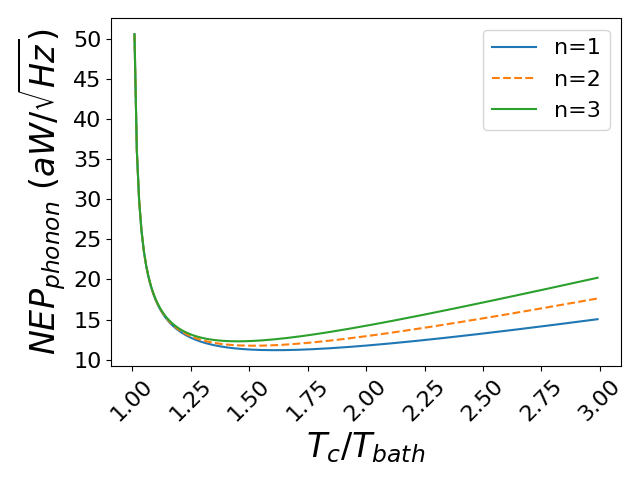
\includegraphics[height=2.5in]{figures/phonon_nep_vs_temperature.png}
\caption[Optimizing critical temperature to minimize phonon noise equivalent power]{Phonon \ac{NEP} as a function of the ratio of critical temperature to bath temperature for three different values of the thermal conductivity power. The goal was to choose $T_{c}$ such that phonon noise was minimized.
\label{fig:phonon_nep_vs_temps} }
\end{center}
\end{figure}

\subsubsection{Thermal Conductance}

%\textcolor{red}{It's not obvious that/why a decrease in radiative load can equate to an increase in detector sensitivity. This needs to be spelled out clearly somewhere. Here?}

%\textcolor{red}{You're talking about radiative loads and thermal conductance and assuming rather than making the connection between them.}

Ground-based telescopes design their detectors to accommodate the radiative load and fluctuations from the atmosphere. 
Long-duration balloon flights, however, typically float at an altitude of $\sim$120,000~ft, above $\sim$98\% of the atmosphere. 
%\textcolor{red}{reference CSBF, website? publication(s)?} 
%IF TIME, COME BACK AND CITE THIS. OR, EVEN BETTER, SHOW OUR OWN DATA!
Without any adjustments to detector fabrication, the photon \ac{NEP} in a space-like environment is improved relative to on the ground because of the decrease in radiative power absorbed, Equation~\ref{eq:photon_nep}. 
The decrease in radiative power also allows for, with adjustment to detector fabrication, a decrease in the phonon \ac{NEP}. 
The smaller radiative load allows for a smaller dynamic range which allows for a smaller $G$, Equation~\ref{eq:gbar}. 
The goal was to minimize $G$, in order to minimize the phonon \ac{NEP}, while keeping $G$ large enough for the detectors to not saturate in the presence of the radiative load at float. 

Table~\ref{tab:target_gbar} summarizes the calculation of the target average thermal conductances. 
For \ac{EBEX} at float, the predicted radiative loads on the detectors were 2.4, 7.3, and 12~pW for the 150, 250, and 410~GHz observation bands. 
Assuming bolometer absorption efficiencies of 0.6, 0.5, and 0.4 for the 150, 250, and 410~GHz bands, the predicted absorbed radiative powers were 1.4, 3.6, and 4.6 pW, respectively.
%not mentioning 410 here because it's not accessible from the ground and one number is sufficient for comparison purporses
The \ac{EBEX} detectors inherited their initial design from ground-based telescopes, \ac{APEX} and the South Pole Telescope. 
At 150~GHz, the expected radiative load was a factor of roughly 10 less than the $\sim$15~pW load observed at 150~GHz by \ac{APEX} \cite{Westbrook2014}. 
In order to take advantage of the decrease in radiative load at float and increase the detector sensitivity, the fabrication goal was to lower the average thermal conductance for the 150~GHz detectors to 20~$pW/K$. 
%by a factor of XXX to 30~$pW/K$. 
%I'D LOVE TO HAVE TIME TO BE MORE QUANTITATIVE ABOUT THE CHANGES RELATIVE TO APEX/SPT
In order to decrease G for the 150~GHz detectors, the spiderweb legs were roughly doubled in length, from 0.5~mm to 1.05~mm, and two of the legs were decreased in width from 17~$\mu m$ to 6~$\mu m$, right panel of Figure~\ref{fig:bolo_and_bling}. 
The average thermal conductance goal for the 250~GHz was 50~$pW/K$ and for the 410~GHz detectors was 60~$pW/K$, Table~\ref{tab:target_gbar}.
This design goal provided a safety factor of 2.5, for all observation frequency bands, in case of unanticipated radiative load or fluctuations.
%IF YOU HAVE TIME, A TABLE WOULD BE REALLY NICE HERE! DONE. 
%IF YOU HAVE TIME, SEARCH FOR OTHER APEX(SZ) PUBLISHED PAPERS WITH MEASURED LOAD
%\textcolor{red}{Is ben's thesis an acceptable place to reference for the APEX measured load?? If not, which published paper is?}

\begin{table}[ht!]
\centering
\begin{tabular}{| c | c | c | c | c | c  |}\hline
Freq (GHz) & $P_{input}$ (pW) & $\epsilon$ & $P_{absorbed}$ (pW) & $\times$ Safety Factor & Target $\overline{G}$ \\ \hline
%150 & 2.4 & 0.6 & 1.4  & 3.6 & 19  \\
%250 & 7.3 & 0.5 & 3.7 & 9.1 & 48  \\  %this predicted Gbar doesn't agree with paper (48 vs 45)
%410 & 12 & 0.4 & 4.7 & 11.6 & 61  \\ \hline  %this predicted Gbar doesn't agree with paper (61 vs 63) 
%rounding errors???
150 & 2.4 & 0.6 & 1.4  & 4 & 19  \\
250 & 7.3 & 0.5 & 3.7 & 9 & 45  \\
410 & 12 & 0.4 & 4.7 & 12 & 63  \\ \hline
\end{tabular}
\caption[Target average thermal conductance calculations]{For each observation frequency, the path to the target average thermal conductance. $P_{input}$ was calculated given all of the predicted transmissions and reflections of all of the optical elements. $\epsilon$ is the detector absorption efficiency assumed. $P_{absorbed}$ is the predicted absorbed power, $P_{input} \cdot \epsilon$. All frequency bands were multiplied by a safety factor of 2.5. The target $\overline{G}$ was $P_{absorbed}/\Delta T$, where $\Delta T$ was the target $T_{crit}$=0.44~K minus the expected $T_{ebex}$=0.25~K.
\label{tab:target_gbar} }
\end{table}



\subsubsection{Time Constant}

%\textcolor{red}{You should talk about time constants... BUT. Your analysis was super simple. And what they did for the paper was much better. So... What do you do? Are you able to write anything intelligent (and correct) about time constants in a small amount of time?}
%
%\textcolor{red}{You really ought to talk about what sets the lower limit (readout) and upper limit (scan speed) on the time constant.}
%
%\textcolor{red}{Also, you can't just say it needs to be held approximately constant if you don't know what the time constants for the ground-based telescopes were!}
%
%\textcolor{red}{Why did we have an observation frequency band dependent target tau??}
%
%\textcolor{red}{I think the following paragraph is not true to how the ideal $\tau$ was decided. Also, isn't $\tau$ also a function of loopgain? (see irwin/hilton p12 on)}
%So long as the thermal conductance between the \ac{TES} and the bath was the dominant effect, the time constant of the bolometer was $\tau = C/G$. 
%When the loopgain was high, though, the time constant was sped up $\tau_{eff} = \tau / ( 1 + \mathscr{L}$.
%

The \ac{TES}' intrinsic thermal time constant was $\tau_0 = C/G$ and it was sped up by electrothermal feedback to give $\tau_{ETF} = \tau_0/(1 + \mathscr{L})$. 
The time constant target was set by the bolometer's LCR filter bandwidth and by the telescope scan speed. 
Relative to the ground-based telescopes, the time constant needed to be held approximately constant because we used the same \ac{DfMUX} electronics and because \ac{EBEX} was to have roughly the same scan speed. 
Since the thermal conductance, G, was decreased relative to the ground-based detector design, in order to keep $\tau$ constant, the heat capacity, C, also needed to be decreased. 
During the fabrication process for the \ac{APEX} ground-based detectors, the bling in the center of the web was made of 500-700~nm of gold \cite{Westbrook2014}. %TOO COMPLICATED. A NICE TO HAVE, NOT A NEED.
For the \ac{EBEX} detectors, we decreased the total thickness of the gold deposited to 20~nm. 
This provided the dominant heat capacity for the detector and was expected to be 0.5~pJ/K for all observation frequency bands. 
%The heat capacity was dominated by this 20~nm gold bling in the center of the web, see Figure~\ref{fig:bolo_and_bling}. 
%The expected heat capacity was 0.5~pJ/K. 
The target time constants at zero loopgain were calculated by taking the ratio of the expected heat capacities to the target thermal conductances.
%We used Equation~\ref{eq:gbar_to_g} and assumed a power of thermal conductivity of 2 to convert the target average thermal conductances (20, 50, 60, for 150, 250, 410~GHz) to target dynamic thermal conductances (30, 80, 90). 
We used Equation~\ref{eq:gbar_to_g} and assumed a power of thermal conductivity of 2 to convert the target average thermal conductances to target dynamic thermal conductances. 
%This gave target time constants of 16, 6, and 5~ms for the 150, 250, and 410~GHz bands, Table~\ref{tab:Design_Params}.  
This gave target time constants of 17, 13, and 10~ms for the 150, 250, and 410~GHz bands, Table~\ref{tab:Design_Params}.  
%\textcolor{red}{Talk to Franky/Shaul. Is this even true???}
%The dominant heat capacity  dominated by gold deposited  was deposited atop the bling, which was 20~nm of gold atop 1~$\mu m$ of silicon nitride. 		




\begin{table}[ht!]
\centering
%\footnotesize
\begin{tabular}{| c | c c | c c | c c |}\hline
\multicolumn{1}{|c}{Band (GHz)}   &  \multicolumn{2}{|c}{150}   & \multicolumn{2}{|c}{250}   & \multicolumn{2}{|c|}{410}  \\% \hline
                                     & Design & Measured & Design & Measured & Design & Measured  \\ \hline
$R_{n}$ ($\Omega$)            & 1.5  & 1.9  & 1.5  & 1.5  & 1.5  & 1.4  \\
$T_{c}$ (K)                        & 0.44 & 0.45 & 0.44 & 0.48 & 0.44 & 0.47  \\
$\overline{G}$ (pW/K)       & 19   & 39 & 45   & 53 & 63   & 63  \\
$\tau_{0}$ (ms)                 & 17 & 88$^\dagger$  & 13  &  46$^\dagger$  &  10 &  57$^\dagger$ \\\hline
%$C$ (pJ/K)*                         & 0.5  & 3.8$^\dagger$ & 0.5  & 3.3$^\dagger$  & 0.5   & 8.4$^\dagger$  \\ \hline
% Wafer Thickness ($\mu$m)   & \multicolumn{2}{|c|}{150}  & \multicolumn{2}{|c|}{90}  & \multicolumn{2}{|c|}{56}  \\
%$\alpha$ (mm)                &  \multicolumn{2}{|c|}{1.05}   & \multicolumn{2}{|c|}{1.0}   &  \multicolumn{2}{|c|}{0.5}  \\
%$\beta$ (mm)                & \multicolumn{2}{|c|}{1.45} & \multicolumn{2}{|c|}{1.0}  & \multicolumn{2}{|c|}{0.5}  \\ \hline
\multicolumn{7}{l}{\footnotesize$^\dagger$ Median of measurements on a single wafer at each frequency; see EBEX Paper Two \cite{EBEXPaper2}.}\\
%\multicolumn{7}{l}{\footnotesize* Calculated from time constant and thermal conductivity.}
\end{tabular}
\caption[Detector parameter targets and median of measurements for normal resistance, critical temperature, average thermal conductance, and time constants]{Designed and measured detector parameters for each of the frequency
bands.  The values in the 'Measured' columns are median values for 
all detectors on the wafers used for flight.  
Description of the measurements, histograms, and further discussion 
of the measured values are given in Chapter~\ref{sec:detector_characterization}.
%For the parameters $\alpha$ and $\beta$, shown in Figure~\ref{fig:Bolometer_Overview} we give the design values. 
%The lithography was generally accurate to within 0.5~$\mu$m.
\label{tab:Design_Params} }
\end{table}




%\emph{FROM EMAIL EXCHANGES WITH BEN.
%We wanted to decrease G, so we roughly doubled the leg length (where you could find space). Do you have pictures of the mask with the original leg length and the final leg length?
%For 150, we pulled out all of the stops we could.  We doubled the length of 7/8 legs from 0.5mm to 1.05 mm. For the 8th leg, we increased it's length by a factor of 3 to 1.45 mm. In addition, we made all the legs expect the one with Nb 6 um wide.  The old design had 2 / 8 with 17 um wide legs. 
%We wanted to decrease Tc, so you messed around with the thickness of the Al layer in our Al/Ti TES sandwich. 
%Specifically we modulate the thickness of the Al (30-50 nm) compared to the Ti layer, which we held at constant thickness (~110nm). More Al means higher Tc and lower Rn (and converse is true).  Technically it's not a sandwhich (that's Shaul's term) it's just a bilayer, Al with Ti on top. Not Al-Ti-Al nor Ti-Al-Ti.
%We wanted to keep the time constant (C/G) the same, so we decreased the heat capacitance by decreasing the thickness of the bling (or we did something else??). 
%So we still had a BLING layer (the waffle pattern at the center of the photos).  However, we didn't add any EXTRA gold here like SPT and APEX had.  The C of the EBEX detectors comes from 20 nm of Gold on a 1um thick layer of Silicon nitride.  Where as the SPT/APEX had the 20nm of gold for the web, the 1 um of Silicon Nitrides, + ~500-700 nm of extra BLING only gold at the center.  Since gold has a large heat capacity, it dominates the total C in the detectors.  I attached a quick memo on this I wrote for Shaul that summarized the changes in heat capacity. 
%Why did we move away from the circle bling design? 
%This is because the waffle pattern has a lower G than the circle so that heat absorbed by the web more efficiently couples to the TES, which ultimately increases optical efficiency (and thus sensitivity) as the TES has time to sense it (i.e it thermalizes) before the heat is dissipated to the bath via the legs.
%Does the CPA track speed control the thickness of the Al in the Al/Ti bilayer?
%Functionally yes.  There are three knobs one could turn: track speed, target power, and argon pressure.  We chose to modulate thickness by varying the track speed while  trying to keep power and pressure constant.
%In the old design, what was the thickness of the other 6 legs?
%The old design had 6, 6 micron wide legs and 2, 17 micron wide legs (one with leads and the one opposite the one with leads). 
%The one with leads also carried the gold heat link.
%> Do you happen to have a schematic that illustrates how we etch the silicon from beneath the silicon nitride? 
%This is my talk from the collab meeting eons ago at McGill.  Pages 7-13 describe the fab process in a cartoon sort of way.  It's the closest thing I have to showing how we release the bolometer structures in presentation form.  If you want the full PPT version let me know.  What basically happens is you etch holes/trenches in the silicon nitride layer and then let the wafer sit in a chamber with XeF2 (Xenon DiFlouride), which etches silicon much much faster than it etches silicon nitride.  The gas finds it's way into the holes and starts digging/etching out the silicon.  After some time a pocket is formed underneath the Silicon nitride (I can make a slide showing this if you need) and the XeF2 starts to isotropically etch (not just down by side to side as well) all of the silicon underneath the structure.  Let me know if you need any more help describing this process. 
%> Did we have the same goal for Tc for each of our wafers?
%> I said it was 1.7 * bath temperature and I think we assumed the bath would be at 270 mK. (giving us a goal of 460 mK)
%> Does this magic number 1.7 change with frequency band?
%Tc = 1.7* Tbath comes from theory for using dieletrics as a thermal bridge.  The plot attached shows that when n = 3, the optimal Tc (the minimum of the dotted lines) is 1.7 * Tbath. However, we used this is a soft criteria and tune our Tc for psat before we did thermal carrier noise.    That means that we basically did have the same target Tc for each wafer, but that was more to tune Psat rather than noise performance.  We did a pretty good job and found that if Tc was around 480-520  we got the Psats we wanted for our 150 and 250/410 GHz wafers (6-8 and 10-12+ pW) for our mask sets. }
%






%%%%%%%%%%%%%%%%%%%%%%%%%%%%%%%%%%%%%%%%%%%%%%%%%%%%%%%%%%%%%%%%%%%%%%%%%%%%%}}}